\documentclass[main.tex]{subfiles}

\begin{document}

% \textcolor{red}{Вводная лекция}

\section{Лекция 16.03.2021 (Донцов Е.В.)}

\subsection{Математическая модель радиальной трещины ГРП}

\includegraphics[width=\textwidth, page=49]{HF_slides_2021.pdf}

Напомню: в случае радиальной геометрии рассматриваем планарную трещину (растёт, например, в плоскости $Oxy$), есть точечный источник и объёмная закачка жидкости $Q_0$; предполагается, что слоёв нет (или эффекты слоёв малы);
радиальная симметрия и задача всё равно одномерная; единственная разница с плоской трещиной в том, что дивергенция потока будет записана в цилиндрических координатах и уравнение упругости будет другим (а именно другое ядро $M$ -- довольно сложная функция -- её можно найти, но важно знать, что она другая).
\\

Уравнения для радиальной и плоской трещин очень похожи: также есть утечки, есть связь потока и градиента давления, есть критерий распространения.

Аналогично, в случае радиальной трещины можем взять уравнение и оценить значения в нём по порядку величины (ввести безразмерные величины).

Но в чём разница с плоской трещиной?

Появился квадрат в первом уравнении перед характерным масштабом длины, т.к. в исходном уравнении изменились расход (он был двухмерный с размерностью м$^2$/с; теперь он трёхмерный с размерностью м$^3$/с) и дельта-функция (она была одномерной с размерностью 1/м; теперь у неё размерность 1/м$^2$).

И такая разница в один характерный масштаб длины даёт совершенно другой ответ для решения.
Такой, так сказать, геометрический фактор.

\includegraphics[width=\textwidth, page=50]{HF_slides_2021.pdf}

Аналогично, можем оценить решение в пределе viscosity-storage (т.е. когда нет трещиностойкости и нет утечек): решаем аналитически и получаем зависимость радиуса, открытия и давления от времени.
Здесь радиус зависит от времени в степени 4/9; в плоской трещине степень была равна 2/3 (т.е. в случае радиальной трещины радиус от времени растёт не так быстро -- что вполне логично: наш блин растекается, площадь становится больше и поэтому скорость роста со временем уменьшается).

Если сравним с более полным (но тоже приближённым) решением, увидим, что добавились численные множители и зависимость от безразмерного радиуса, которые мы не могли найти с помощью обезразмеривания.

\includegraphics[width=\textwidth, page=51]{HF_slides_2021.pdf}

Абсолютно аналогично можно найти приближённое решение; я не буду рассказывать про детали: берём асимптотику, закон сохранения объёма, решаем и получаем приближённое решение (единственная разница будет в интегрировании по объёму за счёт появившегося дополнительного радиуса).

Но сильно изменяется параметрическое пространство и то, как решение себя ведёт.
Здесь сильно другие безразмерные параметры: по оси $Ox$ безразмерное время (оно теперь не зависит от утечек); по очи $Oy$ безразмерные утечки.

Аналогично есть 4 концептуальных предела.

Но важно, что теперь во времени решение может перескакивать от одного предела к другому.
\\

Можно понять на пальцах: когда трещина очень маленькая, то реализуется режим $M$ (скорость распространения относительно большая), далее при продолжении закачки трещина расширяется (скорость распространения становится меньше) и вязкостная диссипация падает, т.е. переходим в режим $K$; если продолжается дальнейший рост трещины, то её площадь ещё больше возрастает и утечки через эту большую площадь начинают доминировать.
\\

Ещё раз: качественно поведение совсем другое, но то, как вы можете использовать параметрическое пространство, идентично тому, что было в плоской трещине, т.е. мы можем посчитать два безразмерных параметра, они дадут нам точку на параметрическом пространстве, из которой вы узнаете текущий режим.

\includegraphics[width=\textwidth, page=52]{HF_slides_2021.pdf}

Для каждого из режимов есть аналитические решения на открытие, радиус и давление.

Из этих всех формул важно знать, как зависит радиус от времени (в степени примерно 1/2, если утечки маленькие, и в степени 1/4, если утечки большие).

Радиусы в режимах $\tilde{M}$ и $\tilde{K}$ одинаковы (определяется только утечками).

\includegraphics[width=\textwidth, page=53]{HF_slides_2021.pdf}

Здесь всё примерно то же самое, что и для плоской трещины: решение переходит от одного к другому (со временем).
То же самое с формой: в режиме трещиностойкости эллиптическое решение.
\\

На самом деле все решения (что для плоской трещины, что для радиальной) -- открытие как функция радиуса -- в самом первом приближении есть эллипсы; при изменении режима этот эллипс немного приплющивается возле кончика.

\includegraphics[width=\textwidth, page=54]{HF_slides_2021.pdf}

Цель графиков, представленных на слайде, показать, что решение плавно переходит от одного к другому.
И мы знаем аналитические решения для пунктирных линий (предельные решения), мы можем их использовать, чтобы оценить полное решение без использования численного расчёта.

Т.е. всё то же самое, что и для плоской трещины.

\includegraphics[width=\textwidth, page=55]{HF_slides_2021.pdf}

Здесь показаны точки в параметрическом пространстве для разных значений входных параметров.

Если возьмём различные полевые условия, различные лабораторные условия, то на параметрическом пространстве реально можем быть везде.

Правда вряд ли будем слишком глубоко в режиме $\tilde{M}$ или $\tilde{K}$ (обычно всё таки возле границы), но влево/вправо между трещиностойкостью и вязкостью очень легко прыгать.
\\

Эффективность = доля жидкости, которая осталась в трещине, после закачки и утечек.

И без расчётов мы знаем, что оба параметра (и трещиностойкость, и вязкость) важны: оба эти параметра влияют на рост трещины.
\\

Slick Water = практически подобна воде, чуть-чуть более вязкая (эффективность около 1/2).
\\

Linear Gel = вязкий гель.

\includegraphics[width=\textwidth, page=56]{HF_slides_2021.pdf}



\includegraphics[width=\textwidth, page=57]{HF_slides_2021.pdf}



\subsection{Математическая модель Перкинса-Керна-Нордгрена (модель PKN)}

\includegraphics[width=\textwidth, page=58]{HF_slides_2021.pdf}

Рассмотрим ещё одну очень важную модель.
Она ещё более важна с точки зрения практики, чем модель радиальной трещины.

Вспомним, что модель плоской трещины легче всего сформулировать и посчитать (она исторически была самой первой моделью), далее усложнили до радиальной модели, и ещё далее усложнили до модели PKN, которую сейчас и будем рассматривать.

Модель PKN (Перкинса-Керна-Нордгрена) тоже одномерная, но она более близка к реальным геометриям.
Ясно, что есть слои, есть разные типы пород и шансы получить радиальную трещину с точки зрения практики малы.

Основные предположения геометрии PKN: есть одна планарная трещина, распространяющаяся симметрично влево и вправо, мы рассматриваем одну сторону; высота трещины постоянна; длина трещины много больше её высоты; вертикальная компонента потока пренебрежимо мала и градиентом давления по оси $Oy$ тоже пренебрегаем (предполагаем, что давление постоянно вдоль оси $Oy$; другими словами, давление является одномерной функцией от $x$); в каждом вертикальном сечении открытие эллиптическое.

Напомню, что эллиптическое открытие как раз соответствует постоянному давлению, т.е. для плоской и радиальной трещины в случае постоянного давления ($K$-режим) открытие трещины эллиптическое.
\\

Используя эти основные предположения, мы сможем по сути усреднить уравнения по оси $Oy$ и получить одномерную систему уравнений для рассматриваемой геометрии вдоль оси $Ox$.

Почему одномерную?

Потому что это старая модель (80-х годов) и тогда ещё не было широкодоступных вычислительных мощностей.

Все одномерные модели можно относительно легко имплементировать, их можно относительно легко анализировать и по ним можно многое понять (быстро посчитать), т.е. одномерные модели имеют свои преимущества.

\includegraphics[width=\textwidth, page=59]{HF_slides_2021.pdf}

Перейдём к выводу уравнений модели PKN.

Стартуем с более общей формулировки для планарной трещины: двухмерный закон сохранения жидкости, связь потока и градиента давления, уравнение упругости и условие распространения.

Что делаем далее?

Используя предположения модели PKN, усредняем уравнения и из двухмерной системы уравнений получаем одномерную.
По сути мы аналитически решаем по вертикали (говорим, что в вертикальном сечении открытие эллиптическое -- это как бы аналитическое решение по вертикали).

Если присмотреться к полученной системе уравнений, то она практически совпадает с системой для плоской трещины.
Единственное, что сильно изменяется, это уравнение упругости.

Таким образом, главное отличие модели PKN и плоской трещины -- это уравнение упругости.

\includegraphics[width=\textwidth, page=60]{HF_slides_2021.pdf}

Давайте более внимательно посмотрим на уравнение упругости для модели PKN, в частности на ядро $G$ этого уравнения.

На слайде приведена явная форма для ядра; $E$ -- это эллиптический интеграл, но его не стоит боятся, т.к. он является регулярной гладкой функцией, которая меняется в пределах от $\pi$/2 до 1.

Т.е. основная зависимость зашита в множителе перед этим эллиптическим интегралом.

Важно, что при $\left|s\right|\gg 1$:
\beq
G(s)\approx\frac{\pi}{2}\text{sign}(s)
\eeq
и тогда под интегралом появляется дельта-функция.
Другими словами, от интеграла остаётся только среднее раскрытие $\bar{w}(x)$.
Это означает, что давление в трещине пропорционально среднему раскрытию.

Физически получили, что вдали от кончика трещины давление будет пропорционально среднему раскрытию.
Это называется локальным уравнением упругости.

Нелокальное уравнение упругости соответствует зависимости давления в точке от интеграла от раскрытия по всей трещине.
Локальное уравнение упругости соответствует зависимости давления в точке от локального раскрытия в этой точке.
\\

При $s\ll1$ (вблизи кончика трещины):
\beq
G(s)\approx\frac{1}{s}
\eeq
и тогда получаем ядро плоской трещины.
\\

Таким образом, получили как бы более общее уравнение упругости, которое описывает поведение трещины возле кончика в форме аналогичной плоской трещине, а при удалении от кончика оно плавно переходит в локальное уравнение упругости.

\includegraphics[width=\textwidth, page=61]{HF_slides_2021.pdf}

Есть два варианта поиска решения для модели PKN:

1) более простое решение, которое опирается на локальную упругость;
говорим, что вдали от кончика применимо локальное уравнение упругости, а возле кончика будем использовать специальные граничные условия (чтобы описать поведение возле кончика), но не будем использовать более сложные уравнения упругости возле кончика (итог: локальное уравнение упругости + специальный критерий распространения на кончике);

2) решение исходного интегрального уравнения упругости честно и численно;
используем честное граничное условие на критерий распространения и честное уравнение упругости (итог: полное уравнение упругости + стандартный критерий распространения).

На графиках приведён пример из статьи.
Показаны графики зависимости открытия от координаты $x$: представлены полная модель planar ILSA, модель PKN с нелокальной упругостью и две модели PKN с локальной упругостью (с различными специальными критериями распространения).
\\

Важно, что при низкой трещиностойкости все решения примерно совпадают вдали от кончика и есть различие лишь возле кончика.

Встаёт вопрос: какую задачу мы хотим решить?
Ведь в зависимости от задачи можем использовать разные методы.

Если задача состоит в том, чтобы оценить общую длину трещины и общее раскрытие, то использовать локальную упругость вполне можно.

Но если мы хотим точно описать поведение возле кончика и в принципе иметь более точное решение, то тогда лучше использовать нелокальную упругость и считать всё численно.

\includegraphics[width=\textwidth, page=62]{HF_slides_2021.pdf}

\includegraphics[width=\textwidth, page=63]{HF_slides_2021.pdf}

\includegraphics[width=\textwidth, page=64]{HF_slides_2021.pdf}

\includegraphics[width=\textwidth, page=65]{HF_slides_2021.pdf}

\includegraphics[width=\textwidth, page=66]{HF_slides_2021.pdf}

\includegraphics[width=\textwidth, page=67]{HF_slides_2021.pdf}

\includegraphics[width=\textwidth, page=68]{HF_slides_2021.pdf}

\includegraphics[width=\textwidth, page=69]{HF_slides_2021.pdf}

\includegraphics[width=\textwidth, page=70]{HF_slides_2021.pdf}

\includegraphics[width=\textwidth, page=71]{HF_slides_2021.pdf}

\includegraphics[width=\textwidth, page=72]{HF_slides_2021.pdf}

\includegraphics[width=\textwidth, page=51]{HF_slides_2022.pdf}


\end{document}